\newtoggle{withbonus} \togglefalse{withbonus} % set true to show bonus points in grade table

% setting underlying course name (Grundlagenfach Mathematik, §-Unterricht, \ldots)
\newcommand{\mycourse}{Grundlagenfach Informatik}
% name of the class
\newcommand{\myclass}{Klasse 2f}
% set date
\newcommand{\mydate}{15. Januar 2025}

\title{\textbf{Prüfung: Theoretische Informatik}}
\author{Thomas Graf\\
	\mycourse, \myclass}
\date{\mydate}
\maketitle
\thispagestyle{headandfoot}

\begin{center}
	\fbox{\parbox{140mm}{\centering
			\begin{itemize}
				\item Dauer der Prüfung: $45$ Minuten
				      %\item \textbf{Zeige in jeder Aufgabe unbedingt Deine Schritte!}
				\item Erlaubte Hilfsmittel:
				      \begin{itemize}
					      \item Schreibzeug
				      \end{itemize}
			\end{itemize}}}
\end{center}
\vspace{10mm}

\begin{center}
	Vorname: \rule{45mm}{0.8pt}\qquad Nachname: \rule{45mm}{0.8pt}
\end{center}
\vspace{20mm}

\begin{center}
	\iftoggle{withbonus} {
		\combinedgradetable[h][questions]
	} {
		\gradetable[h][questions]
	}
\end{center}
\vspace{15mm}
\begin{center}
	Note:
	\vspace{10mm}

	\rule{8mm}{1.2pt}
\end{center}
%\thispagestyle{empty}
\clearpage

\begin{questions}

	\section*{\textcolor{Green}{Theoretische Informatik}}
	\question
	\begin{parts}
		\part[1] Es seien $L_1 := \lrc{\lambda, x, xx}$ und $L_2 := \lrc{x, yx}$ Sprachen über dem Alphabet $\lrc{x, y, z}$. Bestimmen Sie die Anzahl der Elemente in der Menge $L_1L_2$.
		\vspace{3cm}
		\part[1] Es sei $\Sigma$ ein Alphabet. Erklären Sie, warum $\Sigma^*$ eine unendliche Menge ist.
		\vspace{3cm}
		\part[1]
		Geben Sie eine endliche Sprache $L$ an, sodass $\abs{L^2} < \abs{L}^2$.
		\vspace{3cm}
		\part[1]
		Ist die Beziehung $\lr{\lrc{a, b}^*}^2\subseteq \lr{\lrc{a, b}^2}^*$ wahr oder falsch? Begründen Sie Ihre Antwort.
	\end{parts}

	\droptotalpoints
	\clearpage

	\question[2]{\textbf{Knotenüberdeckung}}

	Gegeben ist der Graph in \cref{fig:VC}. Besitzt dieser Graph eine Knotenüberdeckung der Mächtigkeit höchstens $4$? Begründen Sie Ihre Antwort.

	\begin{figure}[H]
		\centering
		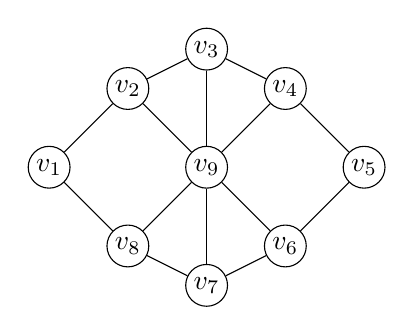
\begin{tikzpicture}[scale=1, every node/.style={circle, draw, fill=white, inner sep=1.5pt}]
			% Nodes
			\node (v1) at (0,0) {$v_1$};       % Bottom-left
			\node (v2) at (1,1) {$v_2$};       % Above v1
			\node (v3) at (2,1.5) {$v_3$};     % Top-middle
			\node (v4) at (3,1) {$v_4$};       % Top-right
			\node (v5) at (4,0) {$v_5$};       % Far-right
			\node (v6) at (3,-1) {$v_6$};      % Bottom-right
			\node (v7) at (2,-1.5) {$v_7$};    % Below-middle
			\node (v8) at (1,-1) {$v_8$};      % Below-left
			\node (v9) at (2,0) {$v_9$};       % Center

			% Edges
			\draw (v1) -- (v2);
			\draw (v2) -- (v3);
			\draw (v3) -- (v4);
			\draw (v4) -- (v5);
			\draw (v5) -- (v6);
			\draw (v6) -- (v7);
			\draw (v7) -- (v8);
			\draw (v8) -- (v1);
			\draw (v2) -- (v9);
			\draw (v3) -- (v9);
			\draw (v4) -- (v9);
			\draw (v6) -- (v9);
			\draw (v7) -- (v9);
			\draw (v8) -- (v9);
		\end{tikzpicture}
		\caption{Entscheidungsproblem zur Knotenüberdeckung.}
		\label{fig:VC}
	\end{figure}
	\clearpage
	\question{\textbf{Endlichen Automaten zeichnen 1}}

	Gegeben ist die Sprache
	\begin{align*}
		L_1 := \setcm{0x101y}{x,y\in\lrc{0,1}^*}.
	\end{align*}
	\begin{parts}
		\vspace{5cm}
		\part[2] Entwerfen Sie einen endlichen Automaten (in Diagrammform), welcher $L_1$ akzeptiert.
	\end{parts}
	\droptotalpoints

	\clearpage
	\question{\textbf{Endlichen Automaten zeichnen 2}}

	Gegeben ist die Sprache \begin{align*} L_2 := \setcm{x1y}{x,y\in\lrc{0,1}^*, \abs{y} = 1}.
	\end{align*}
	\begin{parts}
		\part[1] Nennen Sie ein kürzestes Wort in $L_2$.
		\vspace{5cm}
		\part[3] Entwerfen Sie einen endlichen Automaten (in Diagrammform), welcher $L_2$ akzeptiert. \textcolor{Red}{Achtung}: Beachten Sie, dass $110\in L$ aber $100\notin L$.
	\end{parts}
	\droptotalpoints
	\clearpage

	\question[2]{\textbf{Anzahl der Elemente in einer Sprache bestimmen}}

	Es sei $\Sigma = \lrc{0, 1, 7, 4}$ ein Alphabet und $n$ eine gegebene natürliche Zahl. Bestimmen Sie die Anzahl der verschiedenen Wörter der Länge $n$ über $\Sigma$, welche das Teilwort $0$ enthalten.

	\droptotalpoints
	\clearpage

	\question{\textbf{\red{Nicht reguläre} Sprache}}
	Gegeben sei die Sprache
	\begin{align*}
		L_3 := \setcm{w\$\$w^3}{w\in\lrc{0, 1}^*}
	\end{align*}
	über dem Alphabet $\lrc{0, 1, \$}$.

	Zur Vermeidung von Missverständnissen: Für beispielsweise $w = 011$ ist $w^3$
	gegeben durch:
	\begin{align*}
		w^3 = (011)^3 = 011011011.
	\end{align*}
	\begin{parts}
		\part[1] Nenne genau drei verschiedene Wörter, die in $L_3$ liegen.
		\vspace{3cm}
		\part[3] Zeige, dass $L_3$ \red{nicht regulär} ist.
	\end{parts}

	\droptotalpoints
\end{questions}

\clearpage
(leere Seite für Notizen)
